\subsubsection{Konvoliucija}

Konvoliuciniai neuroniniai tinklai yra vieni populiariausių giliųjų neuroninių tinklų. Pirmą kartą sėkmingai įgyvendintas konvoliucinis neuroninis tinklas yra aprašytas darbe \cite{cnn}. Šis tinklas yra skirtas ranka rašytiems pašto kodams atpažinti. Konvoliucinis neuroninis tinklas -- tai gilusis neuroninis tinklas, kurio bent viename sluoksnyje yra naudojama konvoliucijos operacija, dar vadinama sąsuka. Konvoliucija - tai matematinė operacija, kurios operandai yra dvi funkcijos $f$ ir $g$, ir kurios rezultatas yra funkcija, kuri apibūdina kaip viena funkcija keičia kitą. Ši operacija yra žymima $f * g$ ir ji yra apibrėžiama kaip integralinės transformacijos rūšis pavaizduota formulėje (\ref{eqn:convolution}), kur a ir b nurodo funkcijų  $f$ ir $g$ apibrėžimo sritį.

\begin{equation}
\label{eqn:convolution}
	(f * g)(t) = \int_{a}^{b} f(\tau)g(t - \tau) d\tau
\end{equation}

Konvoliucijos algebros savybės yra komutatyvumas ($f * g = g * f$), asociatyvumas ($f * (g * h) = (f * g) * h$), distributyvumas ($f * (g + h) = (f * g) + (f * h)$), vienetinis elementas $f * \delta = \delta * f = f$ ir daugybos su skaliaru asociatyvumas ($c(f * g) = (cf) * g = f * (cg)$, kur $c \in \R$).

Dažniausiai konvoliuciniuose neuroniniuose tinkluose yra vykdoma konvoliucija diskrečioms funkcijoms. Konvoliucija, kurios operandai yra diskrečios funkcijos yra vadinama diskreti konvoliucija ir ji yra apibrėžiama kaip formulė (\ref{eqn:discrete_convolution}), kur a ir b nurodo funkcijų  $f$ ir $g$ apibrėžimo sritį.

\begin{equation}
\label{eqn:discrete_convolution}
	(f * g)(t) = \sum_{\tau = a}^{b} f(\tau)g(t - \tau)
\end{equation}

Šio magistro baigiamojo darbo tyrimuose yra naudojamos 2D nuotraukos, kurios yra saugomos kaip dviejų dimensijų vaizdai, vadinamos matricomis. Diskreti konvoliucija matricoms yra atliekama naudojantis formulę (\ref{eqn:matrix_convolution}).

\begin{equation}
\label{eqn:matrix_convolution}
	(I * K)(i, j) = \sum_{m} \sum_{n} I(m, n) K(i - m, j - n)
\end{equation}

Konvoliuciniuose neuroniniuose tinkluose matrica $I$ yra vadinama įvestimi, o matrica $K$ - branduoliu arba filtru. Konvoliucija yra komutatyvi, todėl formulė (\ref{eqn:matrix_convolution}) gali būti išreikšta kaip (\ref{eqn:cnn_convolution}).

\begin{equation}
\label{eqn:cnn_convolution}
	(K * I)(i, j) = \sum_{m} \sum_{n} I(i - m, j - n) K(m, n)
\end{equation}

Dažniausiai ši išraiška yra naudojama konvoliuciniuose neuroniniuose tinkluose. Branduolys $K$ dažniausiai yra žymiai mažesnio dydžio nei įvesties matrica $I$ ir $K$ dažniausiai yra išretinta matrica (angl. sparse matrix). Išretinta matrica yra matrica, kurios didžioji dalis elementų yra lygūs 0. Konvoliucijos naudojimas giliuosiuose neuroniniuose patobulina mokymosi procesą dėl konvoliucijos principų - išretintos sąveikos (angl. sparsity), parametrų pasidalinimo ir ekvivalentiško atvaizdavimo.

Paprastame daugiasluoksniame perceptrone kiekvieno sluoksnio visi perceptronai turi po vieną jungtį su tolimesnio sluoksnio kiekvienu perceptronu. Tuo metu konvoliuciniuose tinkluose yra taikoma išretinta sąveika. Išretinta sąveika - tai konvoliucijos padarinys dirbtiniam neuroniniam tinklui, dėl kurios sluoksniuose, kuriuose taikoma konvoliucija, sumažėja jungčių skaičius su tolimesnio sluoksnio perceptronais. Išretintos sąveikos tarp dviejų sluoksnių pavyzdys yra pateiktas \ref{img:sparsity} paveikslėlyje.

\begin{figure}[H]
	\centering
	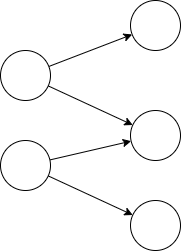
\includegraphics[scale=0.5]{img/sparsity.png}
	\caption{Išretinta sąveika}
	\label{img:sparsity}
\end{figure}

Dėl išretintos sąveikos konvoliuciniai neuroniniai tinklai atsižvelgia tik į reikšmingus požymius. Todėl konvoliucinių neuroninių tinklų mokymas trunka trumpiau ir triukšmas turi mažesnę įtaką rezultatui.

Kitas principas dėl kurio konvoliuciniai neuroniniai tinklai yra spartesni nei daugiasluoksniai perceptronai yra parametrų pasidalinimas. Parametrų pasidalinimas - tai principas, kuriuo remiantis bent vienas parametras yra panaudojamas daugiau nei vienai funkcijai. Konvoliucinių neuroninių tinklų atveju kiekvienas branduolio narys yra naudojamas kiekvienam įvesties nariui. Tuo metu daugiasluoksniame perceptrone, kurio svoriai yra matricos, kiekvienas svorio matricos narys yra naudojamas tik vienam įvesties nariui. Todėl svoriai užima mažiau vietos kompiuterio atmintyje.

Paskutinis principas yra ekvivalentiškumas. Funkcija $f(x)$ yra ekvivalenti funkcijai $g(x)$ jei patenkinama lygybė $f(g(x)) = g(f(x))$. Konvoliucija yra ekvivalenti daugeliui matricos transformacijos funkcijų. Šio principo nauda pasireiškia jei turima nedidelio skaičiaus kaimyninių pikselių funkcija yra naudinga, kai ji yra pritaikoma daugelyje įvesties vietų.
